\documentclass[11pt]{article}
\usepackage[margin=2.5cm]{geometry}
\usepackage{booktabs}
\usepackage{hyperref}
\usepackage{amsmath}
\usepackage[T1]{fontenc}
\usepackage[utf8]{inputenc}
\usepackage{tikz}
\usetikzlibrary{positioning}
\tikzset{every node/.style={circle, draw, minimum size=8mm}}
\begin{document}
\begin{titlepage}
\centering
{\Large Instituto Tecnol\'ogico de Costa Rica\\Escuela de Computaci\'on}\vspace{1cm}
{\huge Proyecto: Reemplazo de Equipos}\vspace{1cm}
{\large II Semestre 2025}\vspace{2cm}
{\large Estudiante(s):}\\Esteban Secaida - Fabian Bustos\vfill
{\large Fecha: \today}
\end{titlepage}
\section*{Datos del Problema}
Costo inicial: $800,00$, Horizonte $T=6$, Vida \'util $L=4$.\\
\textbf{Sin ganancia por uso}.\\
\textbf{Sin inflaci\'on}.\\
\subsection*{Mantenimiento y Reventa por Edad}
\begin{tabular}{c|c|c}\toprule
Edad & Mant. & Reventa\\\midrule
1 & 30,00 & 700,00 \\
2 & 40,00 & 600,00 \\
3 & 80,00 & 300,00 \\
4 & 100,00 & 200,00 \\
\bottomrule\end{tabular}
Se usa $C_{t,x}=\text{Compra}+\sum_{k=1}^{x-t}(\text{Mant}(k))\cdot(1+i)^{k-1}-\text{Reventa}(x-t)\cdot(1+i)^{x-t-1}$ si hay inflaci\'on.\\
\section*{Tabla de $C_{t,x}$}
Entradas v\'alidas con $t<x\le\min(t+L,T)$.

\begin{tabular}{c|c|c}\toprule
 t & x & $C_{t,x}$ \\\midrule
0 & 1 & 130,00 \\
0 & 2 & 270,00 \\
0 & 3 & 650,00 \\
0 & 4 & 850,00 \\
1 & 2 & 130,00 \\
1 & 3 & 270,00 \\
1 & 4 & 650,00 \\
1 & 5 & 850,00 \\
2 & 3 & 130,00 \\
2 & 4 & 270,00 \\
2 & 5 & 650,00 \\
2 & 6 & 850,00 \\
3 & 4 & 130,00 \\
3 & 5 & 270,00 \\
3 & 6 & 650,00 \\
4 & 5 & 130,00 \\
4 & 6 & 270,00 \\
5 & 6 & 130,00 \\
\bottomrule\end{tabular}
\section*{Programaci\'on Din\'amica: $G(t)$ y Siguientes}
\begin{tabular}{c|c|l}\toprule
 t & $G(t)$ & Siguientes \\\midrule
0 & 780,00 & 1 \\
1 & 650,00 & 2 \\
2 & 520,00 & 3 \\
3 & 390,00 & 4 \\
4 & 260,00 & 5 \\
5 & 130,00 & 6 \\
6 & 0,00 &  \\
\bottomrule\end{tabular}
\section*{Todos los planes \`optimos}
Costo m\'inimo total: $G(0)=\mathbf{780,00}$.\\
\noindent Ruta 1: \texttt{0 -> 1 -> 2 -> 3 -> 4 -> 5 -> 6}\\
\section*{Grafos de Rutas \`Optimas}
\subsection*{Ruta óptima 1}
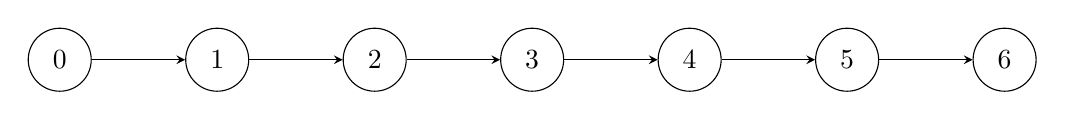
\begin{tikzpicture}[->, >=stealth, node distance=2cm]
\node (R0Y0) at (0,0) {0};
\node (R0Y1) at (2,0) {1};
\node (R0Y2) at (4,0) {2};
\node (R0Y3) at (6,0) {3};
\node (R0Y4) at (8,0) {4};
\node (R0Y5) at (10,0) {5};
\node (R0Y6) at (12,0) {6};
\draw[->] (R0Y0) -- (R0Y1);
\draw[->] (R0Y1) -- (R0Y2);
\draw[->] (R0Y2) -- (R0Y3);
\draw[->] (R0Y3) -- (R0Y4);
\draw[->] (R0Y4) -- (R0Y5);
\draw[->] (R0Y5) -- (R0Y6);
\end{tikzpicture}
\bigskip
\end{document}
